\chapter*{Script Hello World dan Variable }

\begin{enumerate}
	\item menuliskan script hello world di spyder
	\begin{figure} [h]
	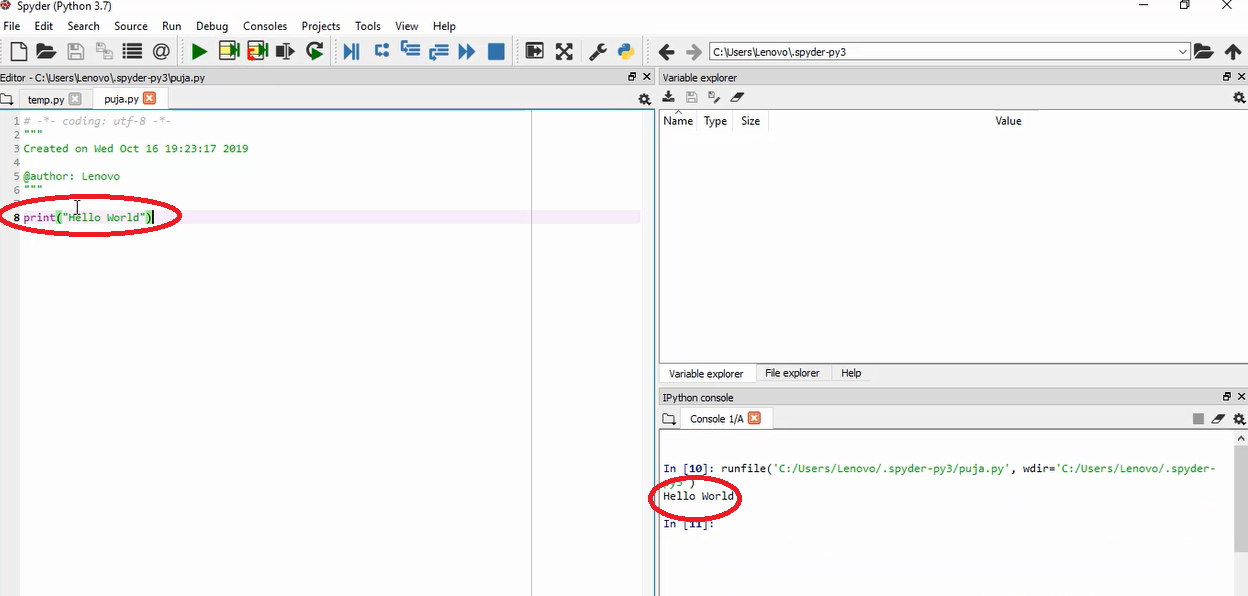
\includegraphics[width=5cm]{variable/4.png}
	\centering
	\end{figure}
	
	\item menuliskan seperti yang ada di gambar disini x merupakan variable dan puja merupakan value 
	\begin{figure} [h]
	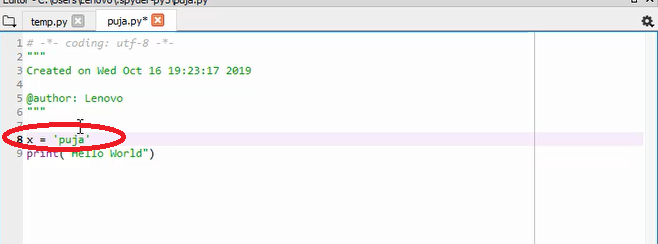
\includegraphics[width=5cm]{variable/1.png}
	\centering
	\end{figure}

	\item Ikuti seperti digambar maksudnya adalah hello + value dari variable yang sudah dibuat sebelumnya  
	\begin{figure} [h]
	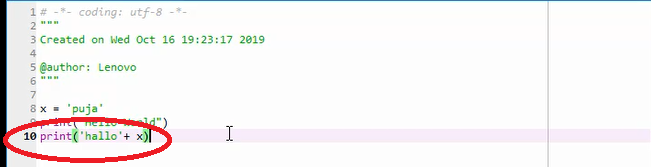
\includegraphics[width=5cm]{variable/2.png}
	\centering
	\end{figure}
	
	\item dan akan jadi seperti yang ada digambar 
	\begin{figure} [h]
	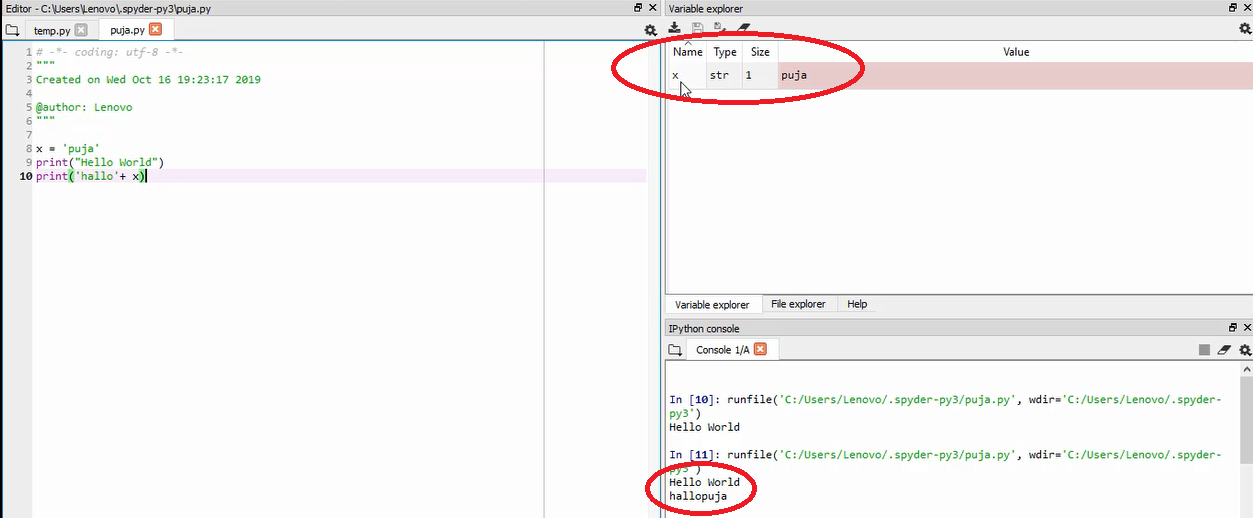
\includegraphics[width=5cm]{variable/3.png}
	\centering
	\end{figure}
	
\end{enumerate}
